\documentclass{article}
\usepackage{icml2025}

\usepackage{microtype}
\usepackage{graphicx}
\usepackage{booktabs}
\usepackage{amsmath,amssymb,amsthm}
\usepackage{mathtools}
\usepackage{tikz}
\usetikzlibrary{positioning,trees,matrix}

\theoremstyle{plain}
\newtheorem{theorem}{Theorem}[section]
\newtheorem{lemma}[theorem]{Lemma}
\newtheorem{proposition}[theorem]{Proposition}
\newtheorem{corollary}[theorem]{Corollary}
\theoremstyle{definition}
\newtheorem{definition}[theorem]{Definition}
\theoremstyle{remark}
\newtheorem{remark}[theorem]{Remark}
\newtheorem{assumption}[theorem]{Assumption}

\icmltitlerunning{Short Title}

\begin{document}

\twocolumn[
\icmltitle{<Full Paper Title>}

\begin{icmlauthorlist}
\icmlauthor{First A. Author}{xxx}
\icmlauthor{Second B. Author}{yyy}
\icmlauthor{Third C. Author}{zzz}
\end{icmlauthorlist}

\icmlaffiliation{xxx}{Affiliation One, City, Country}
\icmlaffiliation{yyy}{Affiliation Two, City, Country}
\icmlaffiliation{zzz}{Affiliation Three, City, Country}

\icmlcorrespondingauthor{First A. Author}{first.last@institution.edu}

\icmlkeywords{Machine Learning, ICML}
\vskip 0.3in
]

\printAffiliationsAndNotice{}

\begin{abstract}
\end{abstract}

\section{Introduction}

\section{Related Work}

\section{Preliminaries and Problem Setup}

\section{Method}
\label{sec:method}

\subsection{Overview}
We propose \emph{Natural Language Edge Labelling} (NLEL), a control layer for structured language-model (LM) reasoning in which each edge carries a natural-language label that specifies \emph{how} the next step should proceed (e.g., ``seek a counterexample'', ``work backward'', ``apply an anthropological lens; probe for defeaters''). A dedicated \emph{tuner} LM reads a tuple $(P,L,C)$---the parent node $P$, the edge label $L$, and the current context $C$---and maps it directly to a control vector $\Pi$ that configures decoding, search, retrieval, and verification for the next expansion.

\subsection{Inputs, Outputs, and Mapping}
\paragraph{Inputs.} $P$ is the current parent state (text and optional structure). $L$ is a free-form natural-language directive for the edge. $C$ denotes the remaining state, which can include the partial tree/graph, concise summaries of the frontier and siblings, budget trackers, and verifier configuration.
\paragraph{Output.} A control vector $\Pi$ whose fields actuate the reasoning stack. A task-agnostic schema can include:
\begin{itemize}
  \item \textbf{Decoding:} temperature, top-$p$, max tokens, repetition penalty;
  \item \textbf{Search:} branch quota, variance/risk coefficient $\beta$, and a UCT/exploration constant;
  \item \textbf{Retrieval:} mixture weights over indices or corpora;
  \item \textbf{Verification:} number and strictness of checks.
\end{itemize}
\paragraph{Mapping.} Let $\Psi : (P,L,C)\mapsto \Pi$ denote the tuner mapping. In our prompt-only instantiation (Section~\ref{subsec:jpe}), $\Psi$ is realized by a JSON parameter emitter that respects a schema with bounds and learns from a compact in-prompt ledger of historical expansions.

\subsection{Expansion Procedure}
We expand the structure in three steps:
\begin{enumerate}
  \item \textbf{Select an edge label $L$.} Labels are natural-language imperatives specifying \emph{how} to think next (e.g., generate a counterexample, analogize, or recurse on a subgoal).
  \item \textbf{Emit control $\Pi = \Psi(P,L,C)$.} The tuner LM consumes $(P,L,C)$ and produces a single control vector adhering to a schema with bounds.
  \item \textbf{Expand under $\Pi$.} Generate or select the child using the actuated settings; update the frontier summaries and budgets in $C$.
\end{enumerate}

% ---------- WIDE FIGURE WITH A LARGER TREE AND CONCRETE LABELS ----------
\begin{figure*}[!t]
  \centering
  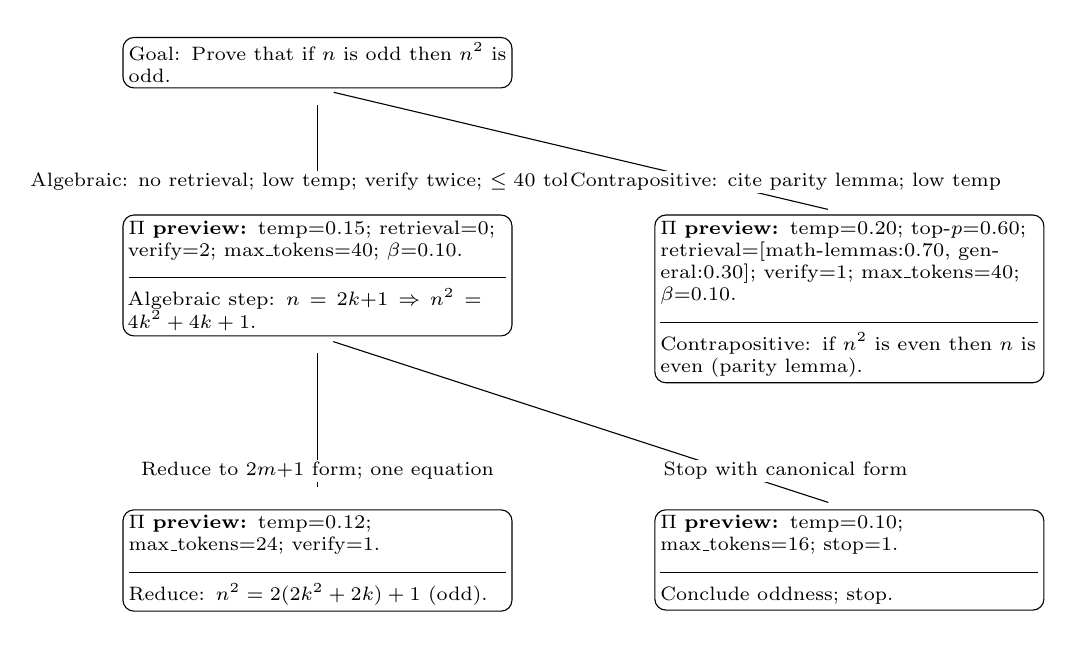
\begin{tikzpicture}[
    node/.style={rectangle, draw, rounded corners, inner sep=2pt, align=left, font=\scriptsize, text width=4.8cm},
    % Two label variants so we can place them above/below and nudge them off the node edge.
    elabelTop/.style={pos=0.88, above, yshift=2pt, fill=white, inner sep=1pt, font=\scriptsize},
    elabelBot/.style={pos=0.88, below, yshift=-2pt, fill=white, inner sep=1pt, font=\scriptsize}
  ]
    %--- Grid with explicit rows: [1, 2, 2] ---
    \matrix[matrix of nodes, row sep=16mm, column sep=18mm] (M) {
      % Row 1 (1 node)
      \node[node] (root) {Goal: Prove that if $n$ is odd then $n^2$ is odd.}; \\
      % Row 2 (2 nodes)
      \node[node] (alg) {%
        \textbf{$\mathrm{\Pi}$ preview:} temp=0.15; retrieval=0; verify=2; max\_tokens=40; $\beta$=0.10.%
        \par\noindent\rule{\linewidth}{0.3pt}\vspace{2pt}\\%
        Algebraic step: $n=2k{+}1 \Rightarrow n^2=4k^2+4k+1$.%
      };
      &
      \node[node] (contra) {%
        \textbf{$\mathrm{\Pi}$ preview:} temp=0.20; top-$p$=0.60; retrieval=[math-lemmas:0.70, general:0.30]; verify=1; max\_tokens=40; $\beta$=0.10.%
        \par\noindent\rule{\linewidth}{0.3pt}\vspace{2pt}\\%
        Contrapositive: if $n^2$ is even then $n$ is even (parity lemma).%
      }; \\
      % Row 3 (2 nodes; both under the SAME parent 'alg')
      \node[node] (alg_reduce) {%
        \textbf{$\mathrm{\Pi}$ preview:} temp=0.12; max\_tokens=24; verify=1.%
        \par\noindent\rule{\linewidth}{0.3pt}\vspace{2pt}\\%
        Reduce: $n^2=2(2k^2+2k)+1$ (odd).%
      };
      &
      \node[node] (alg_stop) {%
        \textbf{$\mathrm{\Pi}$ preview:} temp=0.10; max\_tokens=16; stop=1.%
        \par\noindent\rule{\linewidth}{0.3pt}\vspace{2pt}\\%
        Conclude oddness; stop.%
      }; \\
    };

    %--- Edges (explicit): start at parent.south, end at child.north
    % Shorten near nodes so labels have breathing room and don't overlap the boxes
    \draw[shorten <=6pt, shorten >=8pt] (root.south)
      -- node[elabelTop]{Algebraic: no retrieval; low temp; verify twice; $\leq 40$ tokens}
      (alg.north);

    \draw[shorten <=6pt, shorten >=8pt] (root.south)
      -- node[elabelTop]{Contrapositive: cite parity lemma; low temp}
      (contra.north);

    \draw[shorten <=6pt, shorten >=8pt] (alg.south)
      -- node[elabelTop]{Reduce to $2m{+}1$ form; one equation}
      (alg_reduce.north);

    \draw[shorten <=6pt, shorten >=8pt] (alg.south)
      -- node[elabelTop]{Stop with canonical form}
      (alg_stop.north);
  \end{tikzpicture}
  \caption{Rows of width $[1,2,2]$ with edges drawn explicitly from the bottom of each parent node to the top of the child node. Natural-language edge labels sit on the edges near the child (never adjoining each other). Each child node starts with an upright \emph{$\mathrm{\Pi}$ preview}, then a horizontal separator, then the node’s reasoning content.}
  \label{fig:nlel_schematic}
\end{figure*}
% -----------------------------------------------------------------------

\subsection{Prompt-Only JSON Parameter Emitter (JPE)}
\label{subsec:jpe}
The tuner LM receives three ingredients in the prompt: (i) a concise \emph{schema} that specifies control fields and bounds; (ii) a \emph{historical ledger} of $(P_i,L_i,C_i)\!\mapsto\!\Pi_i$ with outcomes, where rows are tagged as \emph{Pareto} or \emph{dominated} to provide contrastive signals about efficient trade-offs; and (iii) the \emph{current case} $(P,L,C)$. It emits a single JSON object $\Pi$ that must validate against the schema. The ledger can be curated with a lightweight objective that balances task success against compute usage and verification reliability (e.g., success@compute with penalties for excessive tokens or failed checks).

\subsection{Context Features}
To keep $C$ compact and measurable, we surface a small set of features that capture the state of search:
\begin{itemize}
  \item \textbf{Frontier uncertainty:} median $\sigma$ across candidate downstream values (from ensembles, bootstraps, or dropout estimates);
  \item \textbf{Novelty deficit:} median nearest-neighbor distance among frontier candidates (embedding or lexical);
  \item \textbf{Depth:} distance from root (enables exploration annealing and quota schedules);
  \item \textbf{Sibling/frontier summaries:} best $(\mu,\sigma)$ among siblings; counts by edge label; budget usage.
\end{itemize}

\subsection{Downstream Selection (Agnostic to NLEL)}
Given $\Pi$, any downstream planner can be used. A simple variance-aware score combines an estimate of value and uncertainty, for example $S=\mu+\beta\,\sigma$, optionally augmented with a UCT-style exploration term. The specific selector is orthogonal to NLEL; $\Pi$ only sets the knobs.

\subsection{Stability and Safety}
We employ non-intrusive guards: (i) strict schema/bounds validation for emitted JSON; (ii) projection into a trust region around safe defaults to prevent pathological jumps; and (iii) depth-annealed exploration so late-depth expansions remain conservative.

\subsection{Design Notes}
NLEL is compatible with a non-reasoning tuner or a reasoning tuner (e.g., CoT/ToT) used \emph{only} as a controller. The child reasoner can be held fixed to cleanly attribute outcomes to the edge label and the control vector~$\Pi$.

\section{Theory (Optional)}

\section{Experiments}
% TODO: Empirical check for depth annealing (Section 3.7(iii)):
%       Compare depth-annealed exploration vs. no annealing under identical budgets.
%       Measure success@compute and reliability under verification constraints.
% TODO: Ablations on: (a) label vocabularies, (b) tuner type, (c) ledger size.

\section{Limitations}

\section{Conclusion}

\section*{Impact Statement}

% \section*{Acknowledgements}

\bibliographystyle{icml2025}
\bibliography{references}

\appendix

\section{Additional Experimental Details}
\section{Proofs}
\section{Extra Results}

\end{document}
